\chapter{Distributed MPC for Formation Path-Following of Multi-Vehicle Systems}
\label{chap:handpos_MPC}

\pgfplotsset{table/search path={figures/handpos_MPC/data}}

The chapter considers the problem of formation path-following of multiple vehicles and proposes a solution based on combining distributed model predictive control with parametrizations of the trajectories of the vehicles using polynomial splines. Introducing such parametrization leads indeed to two potential benefits: a) reducing the number of optimization variables, and b) enabling enforcing constraints on the vehicles in a computationally efficient way. Moreover, the proposed solution formulates the formation path-following problem as a distributed optimization problem that may then be solved using the alternating direction method of multipliers (ADMM).
The proposed approach is applicable to all vehicles that can be modeled as differentially flat systems.
In this chapter, we present numerical simulations with marine vehicles and differential drive robots.
The contents of this chapter are based on \cite{matous_MPC_2022}.

\section{Introduction}
    
As mentioned in Chapter~\ref{chap:introduction}, the formation path-following problem is commonly solved using two types of methods: leader-follower and coordinated path-following.
Both methods can be implemented using \acrfull{mpc} \cite{wang_path_2021,kanjanawanishkul_distributed_2008}.
These \gls{mpc} schemes are based on sampling (\emph{i.e.,} discretizing the dynamics of the vehicles).
Consequently, any constraints on trajectories or states can only be enforced at discrete time-instances.
In other words, we have no control over the behavior of the system between the samples.
We can mitigate this issue by decreasing the sampling time.
However, by decreasing the sampling time, we increase the number of optimized variables, thus increasing the computational and communication requirements.

In recent years, researchers have focused on computationally tractable \gls{mpc} schemes.
One possibility of reducing the computational requirements is to parametrize the vehicles' trajectories using splines.
\cite{saska_2016_predictive} have proposed a spline-based path planning \gls{mpc} algorithm for first-order nonholonomic vehicles.
The algorithm solves the point-to-point formation tracking problem with static obstacles.
Another spline-based \gls{mpc} algorithm has been proposed by \cite{van_parys_2017_DMPC}.
This algorithm is applicable to a wider range of systems compared to \cite{saska_2016_predictive}, and it has been demonstrated on point-to-point and trajectory tracking problems.
However, there is, to the best of our knowledge, no reported work on how to apply spline-based \gls{mpc} to the coordinated path-following problem.

The goal of this chapter is thus to propose a spline-based \gls{mpc} strategy for the coordinated path-following problem, test its suitability for the purpose, and understand which trade-offs characterize this scheme. As we explain in the next section, spline-based \gls{mpc} imposes some assumptions on the structure of the model of the vehicles.    
The spline-based \gls{mpc} scheme can thus be seen as a trade-off between lower computational requirements and more restrictive assumptions on the model.

The remainder of the paper is organized as follows.
In Section~\ref{sec:problem-description}, we present the general assumptions on the model of the vehicles and formally define the formation path-following problem.
In Section~\ref{sec:spline-based-MPC}, we propose the distributed spline-based \gls{mpc} scheme.
Section~\ref{sec:case_studies} presents two case studies.
Finally, Section~\ref{sec:conclusion} gives some concluding remarks.

\section{Problem Description}
\label{sec:problem-description}

In this section, we first introduce the assumptions on the model of the vehicles.
Then, we define the objective of formation path-following and pose it as an optimization problem.



\subsection{Vehicle Model}
\label{ssec:vehicle-model}



Here, we discuss the dynamics of a single agent in the network. Let $\bm{x} \in \mathbb{R}^{n_{\bm{x}}}$ be the vector of states.
We assume that the state vector includes the position of the agent.
Without loss of generality, let the first $n_{\bm{q}}$ states be the position of the vehicle.
We can then define the position vector of the vehicle as
\begin{equation}
    \bm{q} = \inlinevector{x_1, \ldots, x_{n_{\bm{q}}}}.
\end{equation}
Since vehicles typically move in either two or three dimensions, we assume that $n_{\bm{q}} \in \left\{2,3\right\}$.
Let $\bm{u} \in \mathbb{R}^{n_{\bm{q}}}$ be the vector of control inputs.
We assume the dynamics of the vehicle to be given by an ordinary differential equation
\begin{equation}
    \dot{\bm{x}} = \bm{f} \left(\bm{x}, \bm{u}\right).
\label{equ:dynamics-of-an-agent}
\end{equation}
%where $\bm{f} : \mathbb{R}^{n_{\bm{x}}} \times \mathbb{R}^{n_{\bm{q}}} \mapsto \mathbb{R}^{n_{\bm{x}}}$ 
Note that we assume the number of inputs to be equal to $n_{\bm{q}}$.
In cases where this assumption does not hold because the vehicle is overactuated, we need to reduce the number of inputs by introducing a control allocation scheme (see, \emph{e.g.,} \cite{johansen_control_2013}).

Let $\bm{y} \in \mathbb{R}^{n_{\bm{q}}}$ be the output of the system.
Note that, in general, the output can be different from the position of the vehicle.
However, as discussed in the next paragraph, it must be possible to obtain the position from the output.

We assume the system to be differentially flat \cite{fliess_1995_flatness}, \emph{i.e.}, we assume that the input and state can be determined from the output, its derivatives, and antiderivatives. Moreover, we assume that the relation between the output and the position is polynomial.
In other words, there exist suitable (nonlinear) functions $\bm{\phi}_{\bm{u}}$ and $\bm{\phi}_{\bm{x}}$, and a multidimensional polynomial function $\bm{\phi}_{\bm{q}}$ of suitable dimensions such that, at any time,
%
\begin{align}
    \bm{u} &= \bm{\phi}_{\bm{u}} \left(\bm{y}, \dot{\bm{y}}, \ddot{\bm{y}}, \ldots, \bm{y}^{(r')}\right), \label{eq:phi_u} \\
    \bm{x} &= \bm{\phi}_{\bm{x}} \left(\bm{y}^{(-r'')}, \ldots, \bm{y}, \dot{\bm{y}}, \ddot{\bm{y}}, \ldots, \bm{y}^{(r')}\right), \label{eq:phi_x} \\ 
    \bm{q} &= \bm{\phi}_{\bm{q}} \left(\bm{y}^{(-r'')}, \ldots, \bm{y}, \dot{\bm{y}}, \ddot{\bm{y}}, \ldots, \bm{y}^{(r')}\right), \label{eq:phi_q}
\end{align}
%
where $r'$ and $r''$ are positive integers.

To model the constraints on the dynamics of the vehicle, we use a multidimensional function $\bm{e}$.
The set of feasible states and inputs is given by
\begin{equation}
    \big\{\left(\bm{x}, \bm{u}\right) \big| \bm{e} (\bm{x}, \bm{u}) \geq \bm{0}\big\}
    \label{eq:e}
\end{equation}
where the inequality is defined component-wise.
We assume that substituting \eqref{eq:phi_u}, \eqref{eq:phi_x} into \eqref{eq:e} yields a set of polynomial constraints.
In other words, we assume that there exists a multidimensional polynomial function $\bm{h}$ such that
\begin{equation}
    \bm{e} (\bm{x}, \bm{u})
    \geq
    \bm{0}
    \, \iff \,
    \bm{h} \left( \bm{y}^{(-r'')}, \ldots, \bm{y}^{(r')} \right)
    \geq
    \bm{0}.
\label{equ:constraint-h-geq-0}
\end{equation}



\subsection{Formation Path-Following}
\label{ssec:formation-path-following}



The goal is to control $N$ vehicles, all subject to the dynamics introduced in Section~\ref{ssec:vehicle-model}, so that they move in a prescribed formation while their barycenter follows a given path.
Let $\bm{p} : \mathbb{R} \rightarrow \mathbb{R}^{n_{\bm{q}}}$ be a function that represents this path. We assume that the function is continuously differentiable and its first derivative satisfies
\begin{equation}
    \norm{\frac{\partial \bm{p}(s)}{\partial s}} = 1.
    \label{eq:path_assumption}
\end{equation}
This implies that for every path point $\bm{p}(s)$, we can define a path-tangential coordinate frame and a corresponding rotation matrix $\bm{R}_p(s)$ between the inertial and path-tangential frames (a 2D example is shown in \figref{fig:path}).

Let then $\bm{q}_1(t), \ldots, \bm{q}_N(t)$ be the trajectories of the $N$ vehicles composing the fleet, and let $\Delta \bm{p}_1^p, \ldots, \Delta \bm{p}_N^p$ be the desired  positions of the vehicles in the formation, relative to the barycenter. Using this notation, the desired trajectory for agent $i$ is given by
\begin{equation}
    \bm{q}_{d,i}(s) = \bm{p}(s) + \bm{R}_p(s)\, \Delta \bm{p}_i^p,
\end{equation} 
for a given $s$.
An example formation is shown in \figref{fig:formation}.

The objective of the control system is to steer the actual vehicle positions $\bm{q}_i(t)$ to follow the desired trajectories $\bm{q}_{d,i}$. Ideally, this means that for a given function $s(t)$ we seek the actual positions to be such that
\begin{equation}
    \bm{q}_i(t)
    \equiv
    \bm{q}_{d,i}\big(s(t)\big),
    \quad i = 1, \ldots, N.
    \label{eq:path_goal}
\end{equation} 

Note that the path parameter $s(t)$ from the previous equation can be treated as an additional \emph{degree of freedom} when designing the controller. Consequently, we also need to find a suitable control law for $s(t)$. For this purpose, let $U_d$ be the desired speed of the barycenter of the formation. %It is then possible to use~\eqref{eq:path_assumption} to connect the desired speed of such barycenter with the actual speed of the actual barycenter $U(t)$ by means of
When the vehicles follow the path perfectly, the actual speed of the barycenter is given by
\begin{equation}
    U(t)
    =
    \norm{\dot{\bm{p}} \big( s(t) \big)}
    =
    \norm{\frac{\partial \bm{p}(s)}{\partial s}\,\dot{s}(t) } = \abs{\dot{s}(t)}.
\end{equation}
The equivalence above implies that the path parameter $s(t)$ should thus be chosen such that
\begin{equation}
    \dot{s} \equiv U_d.
    \label{eq:param_goal}
\end{equation}



\subsection{A centralized solution to the path-formation problem}
\label{ssec:}



The problem of finding for each agent $i$ its actuation signal $\bm{u}_i(t)$ that guarantees following the desired path $\bm{q}_{d,i} \big( s(t) \big)$ as close as possible can thanks to~\eqref{eq:phi_u}--\eqref{eq:phi_q} be transformed into the problem of finding a corresponding output trajectory $\bm{y}_i(t)$.

In general, it is not possible to find an output trajectory $\bm{y}_i(t)$ such that \eqref{eq:path_goal} is satisfied, since the dynamics of the agents are constrained by both~\eqref{equ:dynamics-of-an-agent} and~\eqref{equ:constraint-h-geq-0}. This means that at any time $t$, there is a position error
%
\begin{equation}
    \widetilde{\bm{q}}_i(t)
    =
    \bm{q}_i(t)
    -
    \bm{q}_{d,i} \big( s(t) \big) .
    \label{eq:q_tilde}
\end{equation}
%
Thanks to \eqref{eq:phi_q}, we can express $\widetilde{\bm{q}}_i(t)$ in terms of $\bm{y}_i(t)$
\begin{equation}
    \widetilde{\bm{q}}_i(t)
    =
    \bm{\phi}_{\bm{q}}\left(\bm{y}^{(-r'')}(t), \ldots, \bm{y}^{(r')}(t)\right)
    -
    \bm{q}_{d,i} \big( s(t) \big), \label{eq:y_tilde}
\end{equation}
and thus solve the problem by optimizing $\bm{y}_i(t)$ and $s(t)$.

The problem should be cast in a receding horizon fashion to reject potential disturbances as the mission proceeds.     
We thus propose to formulate the \emph{centralized} problem of optimizing a part of the trajectory, i.e., $\bm{y}_i(t:t+T)$, \linebreak $s(t:t+T)$, as that of optimizing the constrained problem
%
\begin{equation}
    \begin{array}{rcl}
        \opt_{ \left\lbrace \bm{y}_i(t:t+T) \right\rbrace, s(t:t+T)}
        &
        \sum_{i=1}^N
        &
        \int_{t}^{t+T}
        \widetilde{\bm{q}}_i\T(\tau) \, \bm{Q}_{\bm{p}} \, \widetilde{\bm{q}}_i(\tau) {\rm d}\tau \\
        &
        & 
        +
        \int_{t}^{t+T} Q_s\,\left(\dot{s}(\tau) - U_d\right)^2 {\rm d}\tau, 
    \end{array}
\label{eq:optimization_centralized}
\end{equation}
with $T$ being the prediction horizon, $\bm{Q}_{\bm{p}}$ and $Q_s$ positive weight matrices, $\widetilde{q}_{i}$ the position error as defined in~\eqref{eq:y_tilde}, and subject to, for every agent $i = 1, \ldots, N$, to the constraints~\ref{constraint:io} to~\ref{constraint:initial-condition} below:
\begin{enumerate}[label=C\arabic*]
    \item the implicit constraint on the inputs and states, \emph{i.e.}, $\bm{h} \left( \bm{y}_i^{(-r'')}(\tau), \ldots, \bm{y}^{(r')}_i(\tau) \right) \geq \bm{0}, \quad \forall \tau \in [t, t + T]$,
    \label{constraint:io}
    \item the constraint on the initial condition of the state of the system, i.e., $\bm{\phi}_{\bm{x}} \left(\bm{y}_i^{(-r'')}(t), \ldots, \bm{y}^{(r')}_i(t)\right) = \bm{x}_{i}(t)$,
    \item the constraint on the initial condition of the path of the agents, \emph{i.e.}, $s(t)$. In other words, $s(t)$ is not a decision variable, while $s(t+\tau)$ for any $\tau > 0$ is.
    \label{constraint:initial-condition}
\end{enumerate}
We note that the variational problem above may not be solvable using off-the-shelf hardware with limited computing power. For this reason, it will be rewritten below.



\subsection{A distributed solution to the path-formation problem}



Before doing this rewriting, we note that it is possible to make \eqref{eq:optimization_centralized} distributed by letting the path parameter $s(t)$ be a local variable (\emph{i.e.}, $s_i(t)$), and adding a synchronization constraint on the set of $s_i(t)$'s. This leads to the local reformulation

\begin{subequations}
    \begin{align}
        \begin{split}
            &\opt_{ \left\lbrace \bm{y}_i(t:t+T), s_i(t:t+T) \right\rbrace }
            \int_{t}^{t+T}
                \widetilde{\bm{q}}_i\T(\tau)
                \, \bm{Q}_{\bm{p}} \, 
                \widetilde{\bm{q}}_i(\tau)
                {\rm d}\tau \\
            & \qquad \qquad \qquad \qquad
            + \int_{t}^{t+T} Q_s \,\left(\dot{s}_i(\tau) - U_d\right)^2 {\rm d}\tau , 
        \end{split} \label{eq:criterion}\\
        & \text{subject to } \, h\left(\bm{y}_i^{(-r'')}(\tau), \ldots, \bm{y}^{(r')}_i(\tau)\right) \geq \bm{0}, \label{eq:constraint_h} \\
        & \phantom{\text{subject to } \,} \phi_{\bm{x}} \left(\bm{y}_i^{(-r'')}(t), \ldots, \bm{y}^{(r')}_i(t)\right) = \bm{x}_{i}(t), \label{eq:constraint_x0} \\
        & \phantom{\text{subject to } \,} s_i(\tau) = s_j(\tau), \quad \forall j, \tau \in [t, t+T] \label{eq:constraint_gamma_s}
    \end{align}
\label{eq:optimization_distributed}

\end{subequations}

\noindent where $j$ is the index of the generic neighbor of agent $i$. This formulation is again only an intermediate step towards the approach proposed in this paper, as explained below. 



\section{A distributed Spline-Based \gls{mpc} approach to the path-formation problem}
\label{sec:spline-based-MPC}



The goal of this section is to show how constraining $\bm{y}_i$ and $s_i$ to be splines enables rewriting the variational problem above in a way that is computationally tractable.

For the sake of readability, we will use the convention for which sans-serif fonts (\emph{e.g.}, $\coefm{y}$) indicate quantities relative to splines, while serif fonts (\emph{e.g.}, $\bm{y}$) indicate trajectories parametrized in time as above. %Moreover, without loss of generality we assume $t = 0$, so that the to-be-designed trajectory is $\bm{y}_i(0:T)$.



\subsection{Spline parametrization}
\label{ssec:spline_param}



Let $\coefm{b} = \inlinevector{\coef{b}_1, \ldots, \coef{b}_n}$ be the vector of basis functions of a B-spline, and let $\coefm{y}_i = \inlinevector{\coefm{y}_{i,1}\T, \ldots, \coefm{y}_{i,n}\T}$ be a generic matrix and $\coefm{s}_i = \inlinevector{\coef{s}_{i,1}, \ldots, \coef{s}_{i,n}}$ a generic vector of spline coefficients. Assume then that the trajectories and path parameters may be expressed as B-splines, i.e., as
%
\begin{align}
    \bm{y}_i(\tau) &= \sum_{l=1}^n \coefm{y}_{i,l}\,\coef{b}_l(\tau) = \coefm{y}_i\T\,\coefm{b}(\tau), \\
    s_i(\tau) &= \sum_{l=1}^n \coef{s}_{i,l}\,\coef{b}_l(\tau) = \coefm{s}_i\T\,\coefm{b}(\tau).
\end{align}
%
This assumption implies the possibility of exploiting the convex hull property
\begin{equation}
    \coefm{y}_i \geq \bm{0} \, \implies \, \bm{y}(\tau) \geq \bm{0},
\end{equation}
that implies that any polynomial constraint on a spline can be replaced by a (stricter) constraint on the spline coefficients.
In other words, by assuming the output to be a spline, we assume that there exists a function $\mathsf{h}$ such that
\begin{equation}
    \mathsf{h}\left(\coefm{y}_i\right) \geq \bm{0}
    \, \implies \,
    h\left(\bm{y}_i^{(-r'')}(\tau), \ldots, \bm{y}^{(r')}_i(\tau)\right) \geq \bm{0}.
\end{equation}

This eventually enables us to rewrite the trajectory optimization problems in Section~\ref{sec:problem-description} as corresponding spline-based \gls{mpc} problems. %In more details,   

%First, we need to locally approximate the path function and the associated rotation matrix using polynomials
To do so, each agent $i$ must locally approximate the path function and the associated rotation matrix as polynomials
\begin{align}
    \bm{p}(s) &\approx \bm{p}_0 + \bm{p}_1\,s + \ldots + \bm{p}_m\,s^m, \\
    \bm{R}_p(s) &\approx \bm{R}_{p,0} + \bm{R}_{p,1}\,s + \ldots + \bm{R}_{p,m}\,s^m,
\end{align}
over an interval $\left[s_i(t), s_i(t) + s_T\right]$, where $t$ is the current time and $s_T$ is chosen such that $s_T \geq U_d T$.
We then need to impose an additional constraint on the path parameter
\begin{equation}
    s_i(t) \leq s_i(\tau) \leq s_i(t) + s_T, \quad \forall \tau \in \left[t, t + T\right], \label{eq:constraint_s_range}
\end{equation}
to ensure that the polynomial approximation is valid.

This approximation transforms the criterion from \eqref{eq:criterion} into a polynomial function.
The optimization problem \eqref{eq:optimization_distributed} can then be reformulated in terms of spline coefficients 
\begin{subequations}
    \begin{align}
            \opt_{\coefm{y}_i, \coefm{s}_i} &\, J_i\left(\coefm{y}_i, \coefm{s}_i\right), \\
        \text{subject to } & \coefm{y}_i \in \coef{Y}_i, \\
        & \coefm{s}_i \in \coef{S}_i, \\
        & \coefm{s}_i = \coefm{s}_j, \quad \forall j = 1, \ldots, N, \label{eq:s_constraint}
    \end{align} \label{eq:optimization_spline} 
\end{subequations}

\noindent where $J_i$ is the objective function from \eqref{eq:criterion}, reformulated using the spline coefficients, and $\coef{Y}_i$ and $\coef{S}_i$ are the sets of feasible coefficients given by \eqref{eq:constraint_h}, \eqref{eq:constraint_x0} and \eqref{eq:constraint_s_range}.

This optimization problem is then solved in discrete time-steps.
Similarly to collocation-based MPC, we can use the results from the previous time-step to ``warm-start'' the optimization problem.
We do this by extrapolating the previous results over the new horizon (see \figref{fig:warm_start}).

\begin{figure}[!htbp]
    \centering
    % This file was created by matlab2tikz.
%
%The latest updates can be retrieved from
%  http://www.mathworks.com/matlabcentral/fileexchange/22022-matlab2tikz-matlab2tikz
%where you can also make suggestions and rate matlab2tikz.
%
\definecolor{mycolor1}{rgb}{0.00000,0.44700,0.74100}%
%
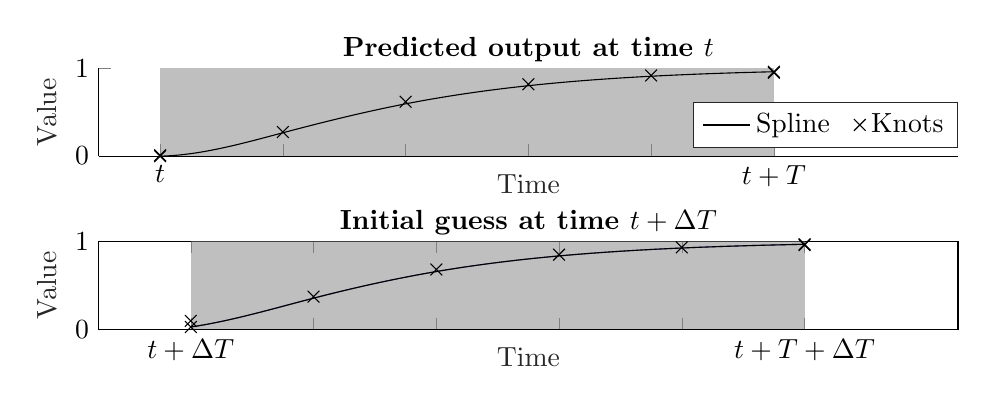
\begin{tikzpicture}

\begin{axis}[%
width=0.9\columnwidth,
height=11.176mm,
at={(0mm,22mm)},
scale only axis,
xmin=-0.5,
xmax=6.5,
xtick={0,1,2,3,4,5},
xticklabels={{$t$},{},{},{},{},{$t+T$}},
xlabel style={font=\color{white!15!black}, yshift=4mm},
xlabel={Time},
ymin=-0.00166163979628464,
ymax=1,
ytick={0,1},
ylabel style={font=\color{white!15!black}},
ylabel={Value},
axis background/.style={fill=white},
title style={font=\bfseries, yshift=-2.5mm},
title={Predicted output at time $t$},
axis x line*=bottom,
axis y line*=left,
legend style={at={(1,0.09)}, anchor=south east, legend cell align=left, align=left, draw=white!15!black},
legend columns=2
]

\addplot[area legend, draw=none, fill=gray, fill opacity=0.5, forget plot]
table[row sep=crcr] {%
x	y\\
0	0\\
5	0\\
5	1\\
0	1\\
}--cycle;
\addplot [color=black]
  table[row sep=crcr]{%
0	-0.00166163979628464\\
0.05	0.000928904578008774\\
0.1	0.00522934423267889\\
0.15	0.0111430974758064\\
0.2	0.0185735826154718\\
0.25	0.0274242179597558\\
0.3	0.0375984218167392\\
0.35	0.0489996124945023\\
0.4	0.0615312083011261\\
0.45	0.075096627544691\\
0.5	0.0895992885332776\\
0.55	0.104942609574967\\
0.6	0.121030008977839\\
0.65	0.137764905049975\\
0.7	0.155050716099455\\
0.75	0.17279086043436\\
0.8	0.190888756362771\\
0.85	0.209247822192768\\
0.9	0.227771476232432\\
0.95	0.246363136789844\\
1	0.264926222173083\\
1.05	0.283378234231657\\
1.1	0.301693008980773\\
1.15	0.319858465977063\\
1.2	0.337862524777161\\
1.25	0.3556931049377\\
1.3	0.373338126015311\\
1.35	0.39078550756663\\
1.4	0.408023169148288\\
1.45	0.425039030316918\\
1.5	0.441821010629153\\
1.55	0.458357029641626\\
1.6	0.474635006910971\\
1.65	0.490642861993819\\
1.7	0.506368514446805\\
1.75	0.52179988382656\\
1.8	0.536924889689719\\
1.85	0.551731451592913\\
1.9	0.566207489092775\\
1.95	0.58034092174594\\
2	0.594119669109039\\
2.05	0.607534672202029\\
2.1	0.620588957898159\\
2.15	0.633288574534004\\
2.2	0.645639570446135\\
2.25	0.657647993971126\\
2.3	0.669319893445549\\
2.35	0.680661317205979\\
2.4	0.691678313588988\\
2.45	0.702376930931148\\
2.5	0.712763217569034\\
2.55	0.722843221839218\\
2.6	0.732622992078274\\
2.65	0.742108576622774\\
2.7	0.751306023809291\\
2.75	0.760221381974399\\
2.8	0.76886069945467\\
2.85	0.777230024586678\\
2.9	0.785335405706996\\
2.95	0.793182891152196\\
3	0.800778529258852\\
3.05	0.808128281705332\\
3.1	0.81523776353718\\
3.15	0.822112503141736\\
3.2	0.82875802890634\\
3.25	0.83517986921833\\
3.3	0.841383552465047\\
3.35	0.84737460703383\\
3.4	0.853158561312019\\
3.45	0.858740943686953\\
3.5	0.864127282545972\\
3.55	0.869323106276414\\
3.6	0.874333943265621\\
3.65	0.879165321900931\\
3.7	0.883822770569683\\
3.75	0.888311817659218\\
3.8	0.892637991556874\\
3.85	0.896806820649992\\
3.9	0.900823833325911\\
3.95	0.90469455797197\\
4	0.908424522975509\\
4.05	0.912018959156592\\
4.1	0.915481907066182\\
4.15	0.918817109687969\\
4.2	0.922028310005639\\
4.25	0.925119251002881\\
4.3	0.928093675663382\\
4.35	0.930955326970832\\
4.4	0.933707947908918\\
4.45	0.936355281461328\\
4.5	0.93890107061175\\
4.55	0.941349058343873\\
4.6	0.943702987641384\\
4.65	0.945966601487972\\
4.7	0.948143642867325\\
4.75	0.95023785476313\\
4.8	0.952252980159076\\
4.85	0.954192762038851\\
4.9	0.956060943386143\\
4.95	0.957861267184641\\
5	0.959597476418031\\
};
\addlegendentry{Spline~~}

\addplot[only marks, mark=x, mark options={}, mark size=3.000pt, draw=black] table[row sep=crcr]{%
x	y\\
0	-0.00166163979628464\\
0	0.00969437911570605\\
1	0.27327001324583\\
2	0.618570718004537\\
3	0.817165129390258\\
4	0.917439939987547\\
5	0.94822814567092\\
5	0.959597476418031\\
};
\addlegendentry{Knots}

\end{axis}

\begin{axis}[%
width=0.9\columnwidth,
height=11.176mm,
at={(0mm,0mm)},
scale only axis,
xmin=-0.5,
xmax=6.5,
xtick={0.25,1.25,2.25,3.25,4.25,5.25},
xticklabels={{$t+\Delta T$},{},{},{},{},{$t+T+\Delta T$}},
xlabel style={font=\color{white!15!black}, yshift=4mm},
xlabel={Time},
ymin=0,
ymax=1,
ytick={0,1},
ylabel style={font=\color{white!15!black}},
ylabel={Value},
axis background/.style={fill=white},
title style={font=\bfseries, yshift=-2.5mm},
title={Initial guess at time $t+\Delta T$}
]
\addplot [color=mycolor1, forget plot]
  table[row sep=crcr]{%
0.25	0.0274242179597558\\
0.3	0.0383688818607485\\
0.35	0.0502727123753448\\
0.4	0.0630713586099857\\
0.45	0.076700469671112\\
0.5	0.0910956946651645\\
0.55	0.106192682698584\\
0.6	0.121927082877812\\
0.65	0.138234544309289\\
0.7	0.155050716099455\\
0.75	0.172311247354752\\
0.8	0.189951787181621\\
0.85	0.207907984686502\\
0.9	0.226115488975836\\
0.95	0.244509949156065\\
1	0.263027014333629\\
1.05	0.281602333614968\\
1.1	0.300171556106525\\
1.15	0.318670330914739\\
1.2	0.337034307146052\\
1.25	0.355199133906904\\
1.3	0.373110469564952\\
1.35	0.390754009532715\\
1.4	0.408125458483927\\
1.45	0.425220521092324\\
1.5	0.442034902031639\\
1.55	0.458564305975608\\
1.6	0.474804437597964\\
1.65	0.490751001572443\\
1.7	0.506399702572779\\
1.75	0.521746245272706\\
1.8	0.53678633434596\\
1.85	0.551515674466274\\
1.9	0.565929970307383\\
1.95	0.580024926543023\\
2	0.593796247846927\\
2.05	0.60723963889283\\
2.1	0.620350804354467\\
2.15	0.633125448905572\\
2.2	0.64555927721988\\
2.25	0.657647993971125\\
2.3	0.669389159554407\\
2.35	0.680787757250281\\
2.4	0.691850626060667\\
2.45	0.702584604987487\\
2.5	0.712996533032658\\
2.55	0.723093249198103\\
2.6	0.732881592485742\\
2.65	0.742368401897494\\
2.7	0.751560516435279\\
2.75	0.760464775101019\\
2.8	0.769088016896632\\
2.85	0.777437080824041\\
2.9	0.785518805885163\\
2.95	0.793340031081921\\
3	0.800907595416234\\
3.05	0.808228337890021\\
3.1	0.815309097505205\\
3.15	0.822156713263704\\
3.2	0.828778024167439\\
3.25	0.83517986921833\\
3.3	0.841368767551858\\
3.35	0.847349958837746\\
3.4	0.853128362879279\\
3.45	0.858708899479738\\
3.5	0.864096488442408\\
3.55	0.869296049570574\\
3.6	0.874312502667517\\
3.65	0.879150767536523\\
3.7	0.883815763980875\\
3.75	0.888312411803856\\
3.8	0.892645630808751\\
3.85	0.896820340798843\\
3.9	0.900841461577415\\
3.95	0.904713912947751\\
4	0.908442614713136\\
4.05	0.912032486676852\\
4.1	0.915488448642184\\
4.15	0.918815420412414\\
4.2	0.922018321790828\\
4.25	0.925102072580708\\
4.3	0.928071357066175\\
4.35	0.930929917454696\\
4.4	0.933681260434576\\
4.45	0.93632889269412\\
4.5	0.938876320921632\\
4.55	0.941327051805416\\
4.6	0.943684592033777\\
4.65	0.945952448295019\\
4.7	0.948134127277447\\
4.75	0.950233135669364\\
4.8	0.952252980159076\\
4.85	0.954197167434887\\
4.9	0.956069204185102\\
4.95	0.957872597098024\\
5	0.959610852861958\\
5.05	0.961287478165209\\
5.1	0.962905979696081\\
5.15	0.964469864142879\\
5.2	0.965982638193907\\
5.25	0.967447808537469\\
};

\addplot[area legend, draw=none, fill=gray, fill opacity=0.5, forget plot]
table[row sep=crcr] {%
x	y\\
0.25	0\\
5.25	0\\
5.25	1\\
0.25	1\\
}--cycle;
\addplot [color=black, forget plot]
  table[row sep=crcr]{%
0.25	0.0274242179597558\\
0.3	0.0383688818607485\\
0.35	0.0502727123753448\\
0.4	0.0630713586099857\\
0.45	0.076700469671112\\
0.5	0.0910956946651645\\
0.55	0.106192682698584\\
0.6	0.121927082877812\\
0.65	0.138234544309289\\
0.7	0.155050716099455\\
0.75	0.172311247354752\\
0.8	0.189951787181621\\
0.85	0.207907984686502\\
0.9	0.226115488975836\\
0.95	0.244509949156065\\
1	0.263027014333629\\
1.05	0.281602333614968\\
1.1	0.300171556106525\\
1.15	0.318670330914739\\
1.2	0.337034307146052\\
1.25	0.355199133906904\\
1.3	0.373110469564952\\
1.35	0.390754009532715\\
1.4	0.408125458483927\\
1.45	0.425220521092324\\
1.5	0.442034902031639\\
1.55	0.458564305975608\\
1.6	0.474804437597964\\
1.65	0.490751001572443\\
1.7	0.506399702572779\\
1.75	0.521746245272706\\
1.8	0.53678633434596\\
1.85	0.551515674466274\\
1.9	0.565929970307383\\
1.95	0.580024926543023\\
2	0.593796247846927\\
2.05	0.60723963889283\\
2.1	0.620350804354467\\
2.15	0.633125448905572\\
2.2	0.64555927721988\\
2.25	0.657647993971125\\
2.3	0.669389159554407\\
2.35	0.680787757250281\\
2.4	0.691850626060667\\
2.45	0.702584604987487\\
2.5	0.712996533032658\\
2.55	0.723093249198103\\
2.6	0.732881592485742\\
2.65	0.742368401897494\\
2.7	0.751560516435279\\
2.75	0.760464775101019\\
2.8	0.769088016896632\\
2.85	0.777437080824041\\
2.9	0.785518805885163\\
2.95	0.793340031081921\\
3	0.800907595416234\\
3.05	0.808228337890021\\
3.1	0.815309097505205\\
3.15	0.822156713263704\\
3.2	0.828778024167439\\
3.25	0.83517986921833\\
3.3	0.841368767551858\\
3.35	0.847349958837746\\
3.4	0.853128362879279\\
3.45	0.858708899479738\\
3.5	0.864096488442408\\
3.55	0.869296049570574\\
3.6	0.874312502667517\\
3.65	0.879150767536523\\
3.7	0.883815763980875\\
3.75	0.888312411803856\\
3.8	0.892645630808751\\
3.85	0.896820340798843\\
3.9	0.900841461577415\\
3.95	0.904713912947751\\
4	0.908442614713136\\
4.05	0.912032486676852\\
4.1	0.915488448642184\\
4.15	0.918815420412414\\
4.2	0.922018321790828\\
4.25	0.925102072580708\\
4.3	0.928071357066175\\
4.35	0.930929917454696\\
4.4	0.933681260434576\\
4.45	0.93632889269412\\
4.5	0.938876320921632\\
4.55	0.941327051805416\\
4.6	0.943684592033777\\
4.65	0.945952448295019\\
4.7	0.948134127277447\\
4.75	0.950233135669364\\
4.8	0.952252980159076\\
4.85	0.954197167434887\\
4.9	0.956069204185102\\
4.95	0.957872597098024\\
5	0.959610852861958\\
5.05	0.961287478165209\\
5.1	0.962905979696081\\
5.15	0.964469864142879\\
5.2	0.965982638193907\\
5.25	0.967447808537469\\
};
\addplot[only marks, mark=x, mark options={}, mark size=3.000pt, draw=black, forget plot] table[row sep=crcr]{%
x	y\\
0.25	0.0274242179597558\\
0.25	0.0970484199353413\\
1.25	0.372765824841548\\
2.25	0.680941786592991\\
3.25	0.84935499261324\\
4.25	0.932717458264032\\
5.25	0.957830892631264\\
5.25	0.967447808537469\\
};
\end{axis}

% \begin{axis}[%
% width=81.29mm,
% height=39.194mm,
% at={(-10.568mm,-5.739mm)},
% scale only axis,
% xmin=0,
% xmax=1,
% ymin=0,
% ymax=1,
% axis line style={draw=none},
% ticks=none,
% axis x line*=bottom,
% axis y line*=left
% ]
% \end{axis}
\end{tikzpicture}%
    
    \caption{Warm-starting the optimization problem. The grey area represents the prediction horizon.}
    \label{fig:warm_start}
\end{figure}



\subsection{ADMM algorithm}



In \cite{boyd_2011_distributed}, it is discussed that ADMM tends to converge to ``modest accuracy'' within a few iterations.
Due to this property, ADMM is often used to solve distributed \gls{mpc} problems.

We assume \emph{synchronous bidirectional reliable} communication.
In other words, we assume that all vehicles exchange information simultaneously and there are no packet losses.
Bidirectional communication implies that the communication network can be described by an undirected graph $\mathcal{G} = \left(\mathcal{V}, \mathcal{E}\right)$, where $\mathcal{V} = \left\{1, 2, \ldots, N\right\}$ correspond to the agents, and $\mathcal{E} \subseteq \mathcal{V}^2$ represents the communication between pairs of agents, \emph{i.e.,} $(i,j) \in \mathcal{E}$ implies that agent $i$ can exchange information with agent $j$. We further assume that $\mathcal{G}$ is connected.

We use relaxed ADMM \cite{bastianello_asynchronous_2021} to solve the problem.
Let $\mathcal{N}_i$ be the set of neighbors of agent $i$.
Relaxed ADMM solves the optimization problem \eqref{eq:optimization_spline} by introducing an auxiliary variable $\coefm{z}_{ji}$ for all $i \in \mathcal{V}, j \in \mathcal{N}_i$.
The optimization problem is then solved iteratively in two steps.
First, we compute $\coefm{y}_i$ and $\coefm{s}_i$ by solving
\begin{equation}
    \coefm{y}_i, \coefm{s}_i
    \leftarrow
    \argmin_{\coefm{y}_i \in \coef{Y}_i, \coefm{s}_i \in \coef{S}_i}
    \mathcal{L}_i
    \left(
        \coefm{y}_i, \coefm{s}_i, \coefm{z}_{ji}
    \right), \label{eq:ADMM_primal_update}
\end{equation}
where $\mathcal{L}_i(\coefm{y}_i, \coefm{s}_i, \coefm{z}_{ji})$ is the augmented Lagrangian given by
\begin{equation}
    \mathcal{L}_i(\coefm{y}_i, \coefm{s}_i, \coefm{z}_{ji}) = J_i(\coefm{y}_i, \coefm{s}_i) - \sum_{j \in \mathcal{N}_i} \coefm{z}_{ji}\T\coefm{s}_i + \frac{\rho}{2}d_i\norm{\coefm{s}_i}^2,
\end{equation}
where $\rho > 0$ is a penalty and $d_i$ is the cardinality of $\mathcal{N}_i$.
In the second step, we update the auxiliary variables
\begin{equation}
    \coefm{z}_{ji} \leftarrow (1 - \alpha) \coefm{z}_{ji} + \alpha \left(2\rho\coefm{s}_j - \coefm{z}_{ij}\right), \label{eq:ADMM_dual_update}
\end{equation}
where $0 < \alpha < 1$ is the step size. To perform this step, each agent $j \in \mathcal{N}_i$ sends a packet
\begin{equation}
    \coefm{w}_{ji} = 2\rho\coefm{s}_i - \coefm{z}_{ji}, \label{eq:ADMM_packet}
\end{equation}
to agent $i$. The update law \eqref{eq:ADMM_dual_update} then becomes
\begin{equation}
    \coefm{z}_{ji} \leftarrow (1 - \alpha) \coefm{z}_{ji} + \alpha \coefm{w}_{ji}. \label{eq:ADMM_dual_update_packet}
\end{equation} 

To further reduce the needed communication bandwidth, we only perform one ADMM iteration per \gls{mpc} step. An overview of the resulting distributed \gls{mpc} is shown in Algorithm \ref{alg:admm}.

\begin{algorithm}[b]
    \caption{ADMM for Distributed MPC}\label{alg:admm}
    \begin{algorithmic}[1]
        \State {\bf Initialization:} Perform several ADMM iterations to get $\coefm{y}_i^0, \coefm{s}_i^0$ and $\coefm{z}_{ij}^0$
        \For{$k = 1,2,\ldots$} every $\Delta T$
            \State Use extrapolation to estimate $\widehat{\coefm{y}}_i^k, \widehat{\coefm{s}}_i^k$ and $\widehat{\coefm{z}}_{ij}^k$
            \State Perform one ADMM iteration using $\widehat{\coefm{y}}_i^k, \widehat{\coefm{s}}_i^k$ and $\widehat{\coefm{z}}_{ij}^k$ as the initial guess
        \EndFor
    \end{algorithmic}
\end{algorithm}



\section{Case Studies}
\label{sec:case_studies}


In this section, we demonstrate the proposed \gls{mpc} scheme on marine vehicles and differential drive robots.
In both cases, the goal is to follow a sine-wave path given by
\begin{equation}
    \bm{p}(s) = \inlinevector{\sigma(s),\; 15\,\sin \left(\frac{\pi}{100}\,\sigma(s)\right)},
\end{equation}
where $\sigma(s)$ is a function chosen such that \eqref{eq:path_assumption} is satisfied and $\sigma(0) = 0$.
This path is then locally approximated using a fifth-order polynomial with $s_T = 75$.

In both case studies, the prediction horizon is set to $50$ seconds.
The path parameter and outputs are represented by cubic splines with $11$ breakpoints.
Consequently, each spline is represented by $13$ coefficients.

In both case studies, we consider a formation of six vehicles.
The formation is chosen such that the vehicles form an equilateral triangle with a side length of $20$ meters.
The desired relative positions of the vehicles, as well as the communication graph are illustrated in \figref{fig:triangle_formation}.


\subsection{Marine vehicles}


In the first case study, we consider marine vehicles with three degrees of freedom.
The model presented in this section describes both autonomous surface vehicles (ASVs) and autonomous underwater vehicles (AUVs) moving in the horizontal plane.
First, let us present the assumptions this model is based on.
\begin{enumerate}[label=A\arabic*]
    \item The vehicles are port-starboard symmetric.
    \item The vehicles are maneuvering at low speeds.
    Consequently, the hydrodynamic damping is linear.
    \item The vehicles are affected by a constant irrotational ocean current.
    Its velocity in the inertial coordinate frame is given by $\bm{V} = \inlinevector{V_x, V_y}$.
\end{enumerate}
Under these assumptions, the model of the vehicle is given by the following differential equations \cite{fossen_handbook_2011}
\begin{subequations}\label{eq:ASV-model}
    \begin{align}
        \dot{x} &= u_{r}\cos\psi - v_{r}\sin\psi + V_x\label{eq:ASV-model-a}\\
        \dot{y} &= u_{r}\sin\psi + v_{r}\cos\psi + V_y\label{eq:ASV-model-b}\\
        \dot{\psi} &= r\label{eq:ASV-model-c}\\
        \dot{u}_{r} &= F_{u_r}(v_{r}) + \tau_{u}\label{eq:ASV-model-d}\\ 
        \dot{v}_{r} &= X(u_{r})r + Y(u_{r})v_{r}\label{eq:ASV-model-e}\\ 
        \dot{r} &= F_{r}(u_{r},v_{r},r) + \tau_{r}\label{eq:ASV-model-f}
    \end{align}
\end{subequations}
where $\eta \triangleq \inlinevector{x, y, \psi}$ is the pose of the vehicle in the {\it North-East-Down} (NED) coordinate frame, $\nu_{r} \triangleq \inlinevector{u_r, v_r, r}$ are the relative (with respect to the ocean current) velocities in the body-fixed coordinate frame, namely the surge velocity, sway velocity, and yaw rate, respectively, and $\tau_{u}$, $\tau_{r}$ are the control inputs.
The functions $F_{u_r}$, $F_{r}$, $X$ and $Y$ represent the Coriolis, centrifugal, and hydrodynamic effects.
Due to space constraints, the definitions of these functions are omitted.
For more details, the reader is referred to \cite{fossen_handbook_2011,borhaug_straight_2007}.

\begin{figure}[b]
    \centering
    \begin{subfigure}[t]{0.15\textwidth}
        \centering
        \def\svgwidth{\textwidth}
        \import{figures/handpos_MPC/}{ASV.pdf_tex}
        \caption{Marine vehicle}
        \label{fig:ASV}
        
    \end{subfigure}
    \begin{subfigure}[t]{0.15\textwidth}
        \centering
        \def\svgwidth{\textwidth}
        \import{figures/handpos_MPC/}{unicycle.pdf_tex}
        \caption{Differential drive robot}
        \label{fig:unicycle}
        
    \end{subfigure}
    \begin{subfigure}[t]{0.143\textwidth}
        \centering
        \def\svgwidth{\textwidth}
        \import{figures/handpos_MPC/}{triangle_formation.pdf_tex}
        \caption{Desired formation}
        \label{fig:triangle_formation}
        
    \end{subfigure}
    \caption{Graphical representations of the vehicles and the formation used in the case studies.}
\end{figure}

Because the vehicle is underactuated (second-order nonholonomic), we cannot use the origin of the body-fixed frame $(x,y)$ as the output of our system.
Instead, we choose a different point, located on the central axis ($x$-axis) of the vehicle, as the output of our system (see \figref{fig:ASV}).
In the literature, this point is referred to as the \emph{hand position} of the vehicle \cite{awton_hand-position-formation_2003,paliotta_trajectory_2019}.
The hand position is defined as
\begin{equation}
    \bm{y} = \inlinevector{x + L\,\cos(\psi), y + L\,\sin(\psi)}, \label{eq:hand}
\end{equation}
where $L > 0$ is the hand length.

The advantage of using the hand position is that we can employ output-feedback linearization to simplify the dynamics.
This procedure follows along the lines of \cite{paliotta_trajectory_2019} with one modification.
In \cite{paliotta_trajectory_2019}, the ocean current is assumed to be unknown.
Here, we assume that the vehicle either can measure the ocean current or employs an observer that provides an accurate estimate of the current (see, \emph{e.g.,} \cite{zhu_kalman_2016}).

We thus introduce the following change of coordinates 
\begin{subequations}
    \begin{align}
        \xi_1 &= x + L\,\cos\psi, \\
        \xi_2 &= y + L\,\sin\psi, \\
        \xi_3 &= u_{r}\cos\psi - v_{r}\sin\psi + V_x - L r\,\cos \psi, \\
        \xi_4 &= u_{r}\sin\psi + v_{r}\cos\psi + V_y + L r\,\sin \psi,
    \end{align}
\end{subequations}
and the following change of inputs 
\begin{equation}
    \begin{bmatrix} \tau_u \\ L\tau_r \end{bmatrix} 
    = 
    \mathfrak{R}(\psi)\T \begin{bmatrix}-F_{\xi_{3}}(\psi, u_r, v_r, r)+u_{1}\\-F_{\xi_{4}}(\psi, u_r, v_r, r)+u_{2}\end{bmatrix}, 
\end{equation}
where $\mathfrak{R} : \mathbb{R} \mapsto {\rm SO}(2)$ denotes the rotation matrix and
\begin{equation}
    \begin{bmatrix}F_{\xi_{3}}(\cdot)\\F_{\xi_{4}}(\cdot)\end{bmatrix}
    = 
    \mathfrak{R}(\psi)\begin{bmatrix}F_{u_r}(\cdot)-v_{r}r-Lr^2 \\ u_{r}r+X(\cdot)r+Y(\cdot)v_{r}+F_r(\cdot)L\end{bmatrix}.
\end{equation}

Using output-feedback linearization, we have simplified the system to a double integrator 
\begin{equation}
    \ddot{\bm{y}} = \bm{u}. 
\end{equation}

\begin{table}[b]
    \begin{center}
    \captionsetup{width=.48\textwidth}
    \caption{Simulation parameters} \label{tab:params}
    
    \begin{subtable}[t]{0.22\textwidth}
        \caption{Marine vehicles}
        \label{tab:ASV}
        
        \begin{tabular}[t]{r|l}
            {\bf Parameter} & {\bf Value} \\
            \hline
            $\Delta T$ & $1$ \\
            $\bm{Q}_p$ & $\begin{bmatrix} 1 & 0 \\ 0 & 1 \end{bmatrix}$ \\
            $Q_s$ & $10$ \\
            $\rho$ & $10$ \\
            $\alpha$ & $0.6$ \\
            $L$ & $1$ \\
            $\bm{V}$ & $\begin{bmatrix} 0.15 \\ 0.1 \end{bmatrix}$
        \end{tabular}
    \end{subtable}
    \begin{subtable}[t]{0.22\textwidth}
        \caption{Differential drive robots}
        \label{tab:unicycle}
        
        \begin{tabular}[t]{r|l}
            {\bf Parameter} & {\bf Value} \\
            \hline
            $\Delta T$ & $0.1$ \\
            $\bm{Q}_p$ & $\begin{bmatrix} 1 & 0 \\ 0 & 1 \end{bmatrix}$ \\
            $Q_s$ & $10$ \\
            $\rho$ & $10$ \\
            $\alpha$ & $0.6$ \\
            $u_{1, \min}$ & $-1$ \\
            $u_{1, \max}$ & $2$ \\
            $u_{2, \min}$ & $-\pi / 8$ \\
            $u_{2, \max}$ & $\pi / 8$
        \end{tabular}
    \end{subtable}
    \end{center}
\end{table}

\begin{figure*}[!htbp]
    \centering
    \begin{subfigure}[c]{0.48\textwidth}
        \centering
        % This file was created by matlab2tikz.
%
%The latest updates can be retrieved from
%  http://www.mathworks.com/matlabcentral/fileexchange/22022-matlab2tikz-matlab2tikz
%where you can also make suggestions and rate matlab2tikz.
%
\definecolor{mycolor1}{rgb}{0.24220,0.15040,0.66030}%
\definecolor{mycolor2}{rgb}{0.27800,0.35560,0.97770}%
\definecolor{mycolor3}{rgb}{0.15400,0.59020,0.92180}%
\definecolor{mycolor4}{rgb}{0.07040,0.74570,0.72580}%
\definecolor{mycolor5}{rgb}{0.50440,0.79930,0.34800}%
\definecolor{mycolor6}{rgb}{0.98710,0.73475,0.24375}%
%
\begin{tikzpicture}

\begin{axis}[%
width=65mm,
height=27.698mm,
at={(0mm,0mm)},
scale only axis,
xmin=-27.7883619793255,
xmax=79.9931504535794,
xlabel style={font=\color{white!15!black}, yshift=1.5mm},
xlabel={$x$-position},
ymin=-15.4431607663429,
ymax=30.4852574604193,
ylabel style={font=\color{white!15!black}},
ylabel={$y$-position},
axis background/.style={fill=white},
title style={font=\bfseries, yshift=-2.75mm},
title={Trajectory},
legend style={at={(0.97,0.03)}, anchor=south east, legend cell align=left, align=left, draw=white!15!black},
]
\addplot [color=black, line width=1.2pt]
  table[]{ASV_trajectory-reference.tsv};
\addlegendentry{Reference path}

\addplot [color=mycolor1, line width=1.0pt]
  table[]{ASV_trajectory-vehicle1.tsv};
\addlegendentry{Vehicles}

\addplot [color=mycolor2, line width=1.0pt]
  table[]{ASV_trajectory-vehicle2.tsv};
%\addlegendentry{Vehicle 2}

\addplot [color=mycolor3, line width=1.0pt]
  table[]{ASV_trajectory-vehicle3.tsv};
%\addlegendentry{Vehicle 3}

\addplot [color=mycolor4, line width=1.0pt]
  table[]{ASV_trajectory-vehicle4.tsv};
%\addlegendentry{Vehicle 4}

\addplot [color=mycolor5, line width=1.0pt]
  table[]{ASV_trajectory-vehicle5.tsv};
%\addlegendentry{Vehicle 5}

\addplot [color=mycolor6, line width=1.0pt]
  table[]{ASV_trajectory-vehicle6.tsv};
%\addlegendentry{Vehicle 6}


\addplot[area legend, line width=1.0pt, draw=black, fill=mycolor1, forget plot]
table[] {ASV_trajectory-vehicle1polygon1.tsv}--cycle;

\addplot[area legend, line width=1.0pt, draw=black, fill=mycolor1, forget plot]
table[] {ASV_trajectory-vehicle1polygon2.tsv}--cycle;

\addplot[area legend, line width=1.0pt, draw=black, fill=mycolor2, forget plot]
table[] {ASV_trajectory-vehicle2polygon1.tsv}--cycle;

\addplot[area legend, line width=1.0pt, draw=black, fill=mycolor2, forget plot]
table[] {ASV_trajectory-vehicle2polygon2.tsv}--cycle;

\addplot[area legend, line width=1.0pt, draw=black, fill=mycolor3, forget plot]
table[] {ASV_trajectory-vehicle3polygon1.tsv}--cycle;

\addplot[area legend, line width=1.0pt, draw=black, fill=mycolor3, forget plot]
table[] {ASV_trajectory-vehicle3polygon2.tsv}--cycle;

\addplot[area legend, line width=1.0pt, draw=black, fill=mycolor4, forget plot]
table[] {ASV_trajectory-vehicle4polygon1.tsv}--cycle;

\addplot[area legend, line width=1.0pt, draw=black, fill=mycolor4, forget plot]
table[] {ASV_trajectory-vehicle4polygon2.tsv}--cycle;

\addplot[area legend, line width=1.0pt, draw=black, fill=mycolor5, forget plot]
table[] {ASV_trajectory-vehicle5polygon1.tsv}--cycle;

\addplot[area legend, line width=1.0pt, draw=black, fill=mycolor5, forget plot]
table[] {ASV_trajectory-vehicle5polygon2.tsv}--cycle;

\addplot[area legend, line width=1.0pt, draw=black, fill=mycolor6, forget plot]
table[] {ASV_trajectory-vehicle6polygon1.tsv}--cycle;

\addplot[area legend, line width=1.0pt, draw=black, fill=mycolor6, forget plot]
table[] {ASV_trajectory-vehicle6polygon2.tsv}--cycle;
\end{axis}

\end{tikzpicture}%
        
    \end{subfigure}
    \begin{subfigure}[c]{0.48\textwidth}
        \centering
        
        % This file was created by matlab2tikz.
%
%The latest updates can be retrieved from
%  http://www.mathworks.com/matlabcentral/fileexchange/22022-matlab2tikz-matlab2tikz
%where you can also make suggestions and rate matlab2tikz.
%
\definecolor{mycolor1}{rgb}{0.24220,0.15040,0.66030}%
\definecolor{mycolor2}{rgb}{0.27800,0.35560,0.97770}%
\definecolor{mycolor3}{rgb}{0.15400,0.59020,0.92180}%
\definecolor{mycolor4}{rgb}{0.07040,0.74570,0.72580}%
\definecolor{mycolor5}{rgb}{0.50440,0.79930,0.34800}%
\definecolor{mycolor6}{rgb}{0.98710,0.73475,0.24375}%
%
\begin{tikzpicture}

\begin{axis}[%
width=65mm,
height=13mm,
at={(0mm,14mm)},
scale only axis,
xmin=0,
xmax=50,
xtick={0,5,10,15,20,25,30,35,40,45,50},
xticklabels={\empty},
ymin=-20.3161212520554,
ymax=0.963323310814234,
ylabel style={font=\color{white!15!black}},
ylabel={$x$-position},
axis background/.style={fill=white},
title style={font=\bfseries, yshift=-2.25mm},
title={Path-following errors},
axis x line*=bottom,
axis y line*=left
]
\addplot [color=mycolor1, line width=1.0pt, forget plot]
  table[]{ASV_errors-1x.tsv};
\addplot [color=mycolor2, line width=1.0pt, forget plot]
  table[]{ASV_errors-2x.tsv};
\addplot [color=mycolor3, line width=1.0pt, forget plot]
  table[]{ASV_errors-3x.tsv};
\addplot [color=mycolor4, line width=1.0pt, forget plot]
  table[]{ASV_errors-4x.tsv};
\addplot [color=mycolor5, line width=1.0pt, forget plot]
  table[]{ASV_errors-5x.tsv};
\addplot [color=mycolor6, line width=1.0pt, forget plot]
  table[]{ASV_errors-6x.tsv};
\end{axis}

\begin{axis}[%
width=65mm,
height=12mm,
at={(0mm,0mm)},
scale only axis,
xmin=0,
xmax=50,
xlabel style={font=\color{white!15!black}},
xlabel={Time},
ymin=-1.45386617375344,
ymax=13.4253597741235,
ylabel style={font=\color{white!15!black}},
ylabel={$y$-position},
axis background/.style={fill=white},
axis x line*=bottom,
axis y line*=left,
legend style={at={(0.99,1.85)}, anchor=north east, legend cell align=left, align=left, draw=white!15!black},
legend columns=2
]
\addplot [color=mycolor1, line width=1.0pt]
  table[]{ASV_errors-1y.tsv};
\addlegendentry{Vehicle 1~}

\addplot [color=mycolor2, line width=1.0pt]
  table[]{ASV_errors-2y.tsv};
\addlegendentry{Vehicle 2}

\addplot [color=mycolor3, line width=1.0pt]
  table[]{ASV_errors-3y.tsv};
\addlegendentry{Vehicle 3}

\addplot [color=mycolor4, line width=1.0pt]
  table[]{ASV_errors-4y.tsv};
\addlegendentry{Vehicle 4}

\addplot [color=mycolor5, line width=1.0pt]
  table[]{ASV_errors-5y.tsv};
\addlegendentry{Vehicle 5}

\addplot [color=mycolor6, line width=1.0pt]
  table[]{ASV_errors-6y.tsv};
\addlegendentry{Vehicle 6}

\end{axis}
\end{tikzpicture}%
        
    \end{subfigure}
    % \begin{subfigure}[c]{0.48\textwidth}
    %     \centering
    %     % This file was created by matlab2tikz.
%
%The latest updates can be retrieved from
%  http://www.mathworks.com/matlabcentral/fileexchange/22022-matlab2tikz-matlab2tikz
%where you can also make suggestions and rate matlab2tikz.
%
\definecolor{mycolor1}{rgb}{0.85000,0.32500,0.09800}%
%
\begin{tikzpicture}

\begin{axis}[%
width=65mm,
height=18.158mm,
at={(0mm,0mm)},
scale only axis,
xmin=0,
xmax=250,
xlabel style={font=\color{white!15!black}},
xlabel={Time},
ymin=0,
ymax=1.2,
ylabel style={font=\color{white!15!black}},
ylabel={Path parameter rate},
axis background/.style={fill=white},
title style={font=\bfseries},
title={Derivative of the path parameter},
legend style={at={(0.99,0.02)}, anchor=south east, legend cell align=left, align=left, draw=white!15!black}
]
\addplot [color=black, line width=1.2pt]
  table[]{ASV_parameter-reference.tsv};
\addlegendentry{Desired path-following speed}

\addplot [color=mycolor1, line width=1.0pt]
  table[]{ASV_parameter-actual.tsv};
\addlegendentry{Mean parameter derivative}

\end{axis}
\end{tikzpicture}%
    % \end{subfigure}
    % \begin{subfigure}[c]{0.48\textwidth}
    %     \centering
    %     % This file was created by matlab2tikz.
%
%The latest updates can be retrieved from
%  http://www.mathworks.com/matlabcentral/fileexchange/22022-matlab2tikz-matlab2tikz
%where you can also make suggestions and rate matlab2tikz.
%
\definecolor{mycolor1}{rgb}{0.24220,0.15040,0.66030}%
\definecolor{mycolor2}{rgb}{0.27800,0.35560,0.97770}%
\definecolor{mycolor3}{rgb}{0.15400,0.59020,0.92180}%
\definecolor{mycolor4}{rgb}{0.07040,0.74570,0.72580}%
\definecolor{mycolor5}{rgb}{0.50440,0.79930,0.34800}%
\definecolor{mycolor6}{rgb}{0.98710,0.73475,0.24375}%
%
\begin{tikzpicture}

\begin{axis}[%
width=65mm,
height=18.158mm,
at={(0mm,0mm)},
scale only axis,
xmin=0,
xmax=250,
xlabel style={font=\color{white!15!black}},
xlabel={$t$ [s]},
ymin=-0.0065,
ymax=0.0100,
ylabel style={font=\color{white!15!black}},
ylabel={Path parameter error},
axis background/.style={fill=white},
title style={font=\bfseries},
title={Constraint satisfaction},
axis x line*=bottom,
axis y line*=left,
%legend style={at={(0.98,0.02)}, anchor=south east, legend cell align=left, align=left, draw=white!15!black},
%legend columns=2
]
\addplot [color=mycolor1, line width=1.0pt]
  table[]{ASV_constraints-1.tsv};
%\addlegendentry{Vehicle 1}

\addplot [color=mycolor2, line width=1.0pt]
  table[]{ASV_constraints-2.tsv};
%\addlegendentry{Vehicle 2}

\addplot [color=mycolor3, line width=1.0pt]
  table[]{ASV_constraints-3.tsv};
%\addlegendentry{Vehicle 3}

\addplot [color=mycolor4, line width=1.0pt]
  table[]{ASV_constraints-4.tsv};
%\addlegendentry{Vehicle 4}

\addplot [color=mycolor5, line width=1.0pt]
  table[]{ASV_constraints-5.tsv};
%\addlegendentry{Vehicle 5}

\addplot [color=mycolor6, line width=1.0pt]
  table[]{ASV_constraints-6.tsv};
%\addlegendentry{Vehicle 6}

\end{axis}
\end{tikzpicture}%
    % \end{subfigure}
    \caption{Results of numerical simulations with six marine vehicles.}
    \label{fig:ASV_simulations}
    
\end{figure*}

Having transformed the system model into the required form, we validated the proposed method in numerical simulations.
The simulations were carried out on a 3DOF model of the light autonomous underwater vehicle (LAUV) developed at the University of Porto \cite{sousa_LAUV_2012}.
The parameters are shown in Table~\ref{tab:ASV}.
The results are shown in \figref{fig:ASV_simulations}.
The left plot shows how the vehicles converge to the desired formation.
The right plot shows the path-following errors $\widetilde{\bm{q}}_i$.
We only show the first 50 seconds since the errors converge to zero afterwards.
% The top-left plot shows how the vehicles converge to the desired formation.
% The top-right plot shows the path-following errors $\widetilde{\bm{q}}_i$.
% We only show the first 50 seconds since the errors converge to zero afterwards.
% The bottom-left plot shows how the derivatives of the path parameter, $\dot{s}_i$, converge to the desired path-following speed.
% Finally, the bottom-right plot shows the satisfaction of constraint \eqref{eq:constraint_gamma_s}.
% Specifically, we show the deviation of individual path parameters from their mean value, \emph{i.e.,} $s_i - 1/N\sum_{j=1}^N s_j$.


\subsection{Differential drive robots}

In the second case study, we consider differential drive robots modeled as unicycles.
The model is given by
\begin{subequations}
    \begin{align}
        \dot{x}_1 &= u_1\,\cos x_3, \\
        \dot{x}_2 &= u_1\,\sin x_3, \\
        \dot{x}_3 &= u_2,
    \end{align} \label{eq:unicycle_ode_x} 
\end{subequations}

\noindent where $x_1, x_2$ give the position, $x_3$ is the orientation of the vehicle, and $u_1$ and $u_2$ are the tangential and angular velocities.

Similarly to the previous case, we could use the hand position to enable the application of the spline-based MPC.
However, doing so would prevent us from imposing constraints on the inputs.
Instead, we will use the procedure from \cite{van_parys_2017_DMPC}.
First, we introduce $z = \tan \frac{x_3}{2}$ and use the following trigonometric identities 
\begin{align}
    \cos x_3 &= \frac{1 - z^2}{1 + z^2}, &
    \sin x_3 &= \frac{2z}{1 + z^2}. 
\end{align}
Next, we substitute $z$ and a modified input $\bar{u}_1 = \frac{u_1}{1 + z^2}$ into the first two lines of \eqref{eq:unicycle_ode_x} to obtain 
\begin{align}
    \dot{x}_1 &= \bar{u}_1 \left(1 - z^2\right), &
    \dot{x}_2 &= 2 \bar{u}_1 z. 
\end{align}
We choose $\bm{y} = \inlinevector{\bar{u}_1, z}$ as the output of the system.
The states and inputs can then be expressed as 
\begin{subequations}
    \begin{align}
        x_1(t) &= \int_{0}^t y_1(\tau) \left(1 - y_2^2(\tau)\right)\, {\rm d}\tau + x_1(0), \\
        x_2(t) &= \int_{0}^t 2 y_1(\tau) y_2(\tau)\, {\rm d}\tau + x_2(0), \\
        x_3(t) &= 2 \arctan y_2(t), \\
        u_1(t) &= y_1(t) \left(1 + y_2^2(t)\right), \label{eq:unicycle_u1} \\
        u_2(t) &= \frac{2 \dot{y}_2(t)}{1 + y_2^2(t)}. \label{eq:unicycle_u2}
    \end{align} \label{eq:unicycle_transform} 
\end{subequations}
Let us assume that there are no constraints on the states and the constraints on the inputs are given by
\begin{align}
    u_{1, \min} &\leq u_1(t) \leq u_{1, \max}, &
    u_{2, \min} &\leq u_2(t) \leq u_{2, \max},
\end{align}
From \eqref{eq:unicycle_u1}, \eqref{eq:unicycle_u2}, the constraints can be expressed as
\begin{subequations}
    \begin{align}
        u_{1, \min} &\leq y_1(t) \left(1 + y_2^2(t)\right) \leq u_{1, \max}, \\
        u_{2, \min}\left(1 + y_2^2(t)\right) &\leq 2 \dot{y}_2(t) \leq u_{2, \max}\left(1 + y_2^2(t)\right).
    \end{align}
\end{subequations}
We have thus shown how to express the states, inputs and constraints in terms of the outputs.

\begin{figure*}[t]
    \centering
    \begin{subfigure}{0.48\textwidth}
        \centering
        % This file was created by matlab2tikz.
%
%The latest updates can be retrieved from
%  http://www.mathworks.com/matlabcentral/fileexchange/22022-matlab2tikz-matlab2tikz
%where you can also make suggestions and rate matlab2tikz.
%
\definecolor{mycolor1}{rgb}{0.24220,0.15040,0.66030}%
\definecolor{mycolor2}{rgb}{0.27800,0.35560,0.97770}%
\definecolor{mycolor3}{rgb}{0.15400,0.59020,0.92180}%
\definecolor{mycolor4}{rgb}{0.07040,0.74570,0.72580}%
\definecolor{mycolor5}{rgb}{0.50440,0.79930,0.34800}%
\definecolor{mycolor6}{rgb}{0.98710,0.73475,0.24375}%
%
\begin{tikzpicture}

\begin{axis}[%
width=65mm,
height=27.698mm,
at={(0mm,0mm)},
scale only axis,
xmin=-28.1494884129424,
xmax=99.9606025384325,
xlabel style={font=\color{white!15!black}, yshift=1.5mm},
xlabel={$ x$ [m]},
ymin=-21.1599330605055,
ymax=33.4310056449558,
ylabel style={font=\color{white!15!black}, yshift=-2.5mm},
ylabel={$ y$ [m]},
axis background/.style={fill=white},
title style={font=\bfseries, yshift=-2.75mm},
title={Trajectory},
legend style={at={(0.98,0.01)}, anchor=south east, legend cell align=left, align=left, draw=white!15!black},
legend columns=2,
]
\addplot [color=black, line width=1.2pt]
  table[]{unicycle_trajectory-1.tsv};
\addlegendentry{Reference path~}

\addplot [color=mycolor1, line width=1.0pt]
  table[]{unicycle_trajectory-2.tsv};
\addlegendentry{Vehicles}

\addplot [color=mycolor2, line width=1.0pt]
  table[]{unicycle_trajectory-3.tsv};
%\addlegendentry{Vehicle 2}

\addplot [color=mycolor3, line width=1.0pt]
  table[]{unicycle_trajectory-4.tsv};
%\addlegendentry{Vehicle 3}

\addplot [color=mycolor4, line width=1.0pt]
  table[]{unicycle_trajectory-5.tsv};
%\addlegendentry{Vehicle 4}

\addplot [color=mycolor5, line width=1.0pt]
  table[]{unicycle_trajectory-6.tsv};
%\addlegendentry{Vehicle 5}

\addplot [color=mycolor6, line width=1.0pt]
  table[]{unicycle_trajectory-7.tsv};
%\addlegendentry{Vehicle 6}


\addplot[area legend, line width=1.0pt, draw=black, fill=mycolor1, forget plot]
table[] {unicycle_trajectory-8.tsv}--cycle;

\addplot[area legend, draw=none, fill=black, forget plot]
table[] {unicycle_trajectory-9.tsv}--cycle;

\addplot[area legend, draw=none, fill=black, forget plot]
table[] {unicycle_trajectory-10.tsv}--cycle;
\addplot [color=black, line width=1.5pt, forget plot]
  table[]{unicycle_trajectory-11.tsv};

\addplot[area legend, line width=1.0pt, draw=black, fill=mycolor1, forget plot]
table[] {unicycle_trajectory-12.tsv}--cycle;

\addplot[area legend, draw=none, fill=black, forget plot]
table[] {unicycle_trajectory-13.tsv}--cycle;

\addplot[area legend, draw=none, fill=black, forget plot]
table[] {unicycle_trajectory-14.tsv}--cycle;
\addplot [color=black, line width=1.5pt, forget plot]
  table[]{unicycle_trajectory-15.tsv};

\addplot[area legend, line width=1.0pt, draw=black, fill=mycolor2, forget plot]
table[] {unicycle_trajectory-16.tsv}--cycle;

\addplot[area legend, draw=none, fill=black, forget plot]
table[] {unicycle_trajectory-17.tsv}--cycle;

\addplot[area legend, draw=none, fill=black, forget plot]
table[] {unicycle_trajectory-18.tsv}--cycle;
\addplot [color=black, line width=1.5pt, forget plot]
  table[]{unicycle_trajectory-19.tsv};

\addplot[area legend, line width=1.0pt, draw=black, fill=mycolor2, forget plot]
table[] {unicycle_trajectory-20.tsv}--cycle;

\addplot[area legend, draw=none, fill=black, forget plot]
table[] {unicycle_trajectory-21.tsv}--cycle;

\addplot[area legend, draw=none, fill=black, forget plot]
table[] {unicycle_trajectory-22.tsv}--cycle;
\addplot [color=black, line width=1.5pt, forget plot]
  table[]{unicycle_trajectory-23.tsv};

\addplot[area legend, line width=1.0pt, draw=black, fill=mycolor3, forget plot]
table[] {unicycle_trajectory-24.tsv}--cycle;

\addplot[area legend, draw=none, fill=black, forget plot]
table[] {unicycle_trajectory-25.tsv}--cycle;

\addplot[area legend, draw=none, fill=black, forget plot]
table[] {unicycle_trajectory-26.tsv}--cycle;
\addplot [color=black, line width=1.5pt, forget plot]
  table[]{unicycle_trajectory-27.tsv};

\addplot[area legend, line width=1.0pt, draw=black, fill=mycolor3, forget plot]
table[] {unicycle_trajectory-28.tsv}--cycle;

\addplot[area legend, draw=none, fill=black, forget plot]
table[] {unicycle_trajectory-29.tsv}--cycle;

\addplot[area legend, draw=none, fill=black, forget plot]
table[] {unicycle_trajectory-30.tsv}--cycle;
\addplot [color=black, line width=1.5pt, forget plot]
  table[]{unicycle_trajectory-31.tsv};

\addplot[area legend, line width=1.0pt, draw=black, fill=mycolor4, forget plot]
table[] {unicycle_trajectory-32.tsv}--cycle;

\addplot[area legend, draw=none, fill=black, forget plot]
table[] {unicycle_trajectory-33.tsv}--cycle;

\addplot[area legend, draw=none, fill=black, forget plot]
table[] {unicycle_trajectory-34.tsv}--cycle;
\addplot [color=black, line width=1.5pt, forget plot]
  table[]{unicycle_trajectory-35.tsv};

\addplot[area legend, line width=1.0pt, draw=black, fill=mycolor4, forget plot]
table[] {unicycle_trajectory-36.tsv}--cycle;

\addplot[area legend, draw=none, fill=black, forget plot]
table[] {unicycle_trajectory-37.tsv}--cycle;

\addplot[area legend, draw=none, fill=black, forget plot]
table[] {unicycle_trajectory-38.tsv}--cycle;
\addplot [color=black, line width=1.5pt, forget plot]
  table[]{unicycle_trajectory-39.tsv};

\addplot[area legend, line width=1.0pt, draw=black, fill=mycolor5, forget plot]
table[] {unicycle_trajectory-40.tsv}--cycle;

\addplot[area legend, draw=none, fill=black, forget plot]
table[] {unicycle_trajectory-41.tsv}--cycle;

\addplot[area legend, draw=none, fill=black, forget plot]
table[] {unicycle_trajectory-42.tsv}--cycle;
\addplot [color=black, line width=1.5pt, forget plot]
  table[]{unicycle_trajectory-43.tsv};

\addplot[area legend, line width=1.0pt, draw=black, fill=mycolor5, forget plot]
table[] {unicycle_trajectory-44.tsv}--cycle;

\addplot[area legend, draw=none, fill=black, forget plot]
table[] {unicycle_trajectory-45.tsv}--cycle;

\addplot[area legend, draw=none, fill=black, forget plot]
table[] {unicycle_trajectory-46.tsv}--cycle;
\addplot [color=black, line width=1.5pt, forget plot]
  table[]{unicycle_trajectory-47.tsv};

\addplot[area legend, line width=1.0pt, draw=black, fill=mycolor6, forget plot]
table[] {unicycle_trajectory-48.tsv}--cycle;

\addplot[area legend, draw=none, fill=black, forget plot]
table[] {unicycle_trajectory-49.tsv}--cycle;

\addplot[area legend, draw=none, fill=black, forget plot]
table[] {unicycle_trajectory-50.tsv}--cycle;
\addplot [color=black, line width=1.5pt, forget plot]
  table[]{unicycle_trajectory-51.tsv};

\addplot[area legend, line width=1.0pt, draw=black, fill=mycolor6, forget plot]
table[] {unicycle_trajectory-52.tsv}--cycle;

\addplot[area legend, draw=none, fill=black, forget plot]
table[] {unicycle_trajectory-53.tsv}--cycle;

\addplot[area legend, draw=none, fill=black, forget plot]
table[] {unicycle_trajectory-54.tsv}--cycle;
\addplot [color=black, line width=1.5pt, forget plot]
  table[]{unicycle_trajectory-55.tsv};
\end{axis}

\end{tikzpicture}%
        
    \end{subfigure}
    \begin{subfigure}{0.48\textwidth}
        \centering
        % This file was created by matlab2tikz.
%
%The latest updates can be retrieved from
%  http://www.mathworks.com/matlabcentral/fileexchange/22022-matlab2tikz-matlab2tikz
%where you can also make suggestions and rate matlab2tikz.
%
\definecolor{mycolor1}{rgb}{0.24220,0.15040,0.66030}%
\definecolor{mycolor2}{rgb}{0.27800,0.35560,0.97770}%
\definecolor{mycolor3}{rgb}{0.15400,0.59020,0.92180}%
\definecolor{mycolor4}{rgb}{0.07040,0.74570,0.72580}%
\definecolor{mycolor5}{rgb}{0.50440,0.79930,0.34800}%
\definecolor{mycolor6}{rgb}{0.98710,0.73475,0.24375}%
%
\begin{tikzpicture}

\begin{axis}[%
width=65mm,
height=11.049mm,
at={(0mm,13.303mm)},
scale only axis,
xmin=0,
xmax=30,
xtick={0,5,10,15,20,25,30},
xticklabels={\empty},
ymin=-22.1017150590729,
ymax=0.481195601357118,
ylabel style={font=\color{white!15!black}},
ylabel={$x$-position},
axis background/.style={fill=white},
title style={font=\bfseries, yshift=-2.25mm},
title={Path-following errors},
axis x line*=bottom,
axis y line*=left
]
\addplot [color=mycolor1, line width=1.0pt, forget plot]
  table[]{unicycle_errors-1.tsv};
\addplot [color=mycolor2, line width=1.0pt, forget plot]
  table[]{unicycle_errors-2.tsv};
\addplot [color=mycolor3, line width=1.0pt, forget plot]
  table[]{unicycle_errors-3.tsv};
\addplot [color=mycolor4, line width=1.0pt, forget plot]
  table[]{unicycle_errors-4.tsv};
\addplot [color=mycolor5, line width=1.0pt, forget plot]
  table[]{unicycle_errors-5.tsv};
\addplot [color=mycolor6, line width=1.0pt, forget plot]
  table[]{unicycle_errors-6.tsv};
\end{axis}

\begin{axis}[%
width=65mm,
height=11.049mm,
at={(0mm,0mm)},
scale only axis,
xmin=0,
xmax=30,
xlabel style={font=\color{white!15!black}},
xlabel={Time},
ymin=-0.975792086286581,
ymax=12.8616127883084,
ylabel style={font=\color{white!15!black}},
ylabel={$y$-position},
axis background/.style={fill=white},
axis x line*=bottom,
axis y line*=left,
legend style={at={(1.05,0.4)}, anchor=south east, legend cell align=left, align=left, draw=white!15!black},
legend columns=2
]
\addplot [color=mycolor1, line width=1.0pt]
  table[]{unicycle_errors-7.tsv};
\addlegendentry{Vehicle 1}

\addplot [color=mycolor2, line width=1.0pt]
  table[]{unicycle_errors-8.tsv};
\addlegendentry{Vehicle 2}

\addplot [color=mycolor3, line width=1.0pt]
  table[]{unicycle_errors-9.tsv};
\addlegendentry{Vehicle 3}

\addplot [color=mycolor4, line width=1.0pt]
  table[]{unicycle_errors-10.tsv};
\addlegendentry{Vehicle 4}

\addplot [color=mycolor5, line width=1.0pt]
  table[]{unicycle_errors-11.tsv};
\addlegendentry{Vehicle 5}

\addplot [color=mycolor6, line width=1.0pt]
  table[]{unicycle_errors-12.tsv};
\addlegendentry{Vehicle 6}
\end{axis}

\end{tikzpicture}%
        
    \end{subfigure}
    \caption{Results of numerical simulations with six differential drive robots.}
    \label{fig:unicycle_simulations}
    
\end{figure*}

The results of numerical simulations are shown in \figref{fig:unicycle_simulations}.
The parameters are shown in Table~\ref{tab:unicycle}.
Due to the numerical inaccuracies caused by \eqref{eq:unicycle_transform} and arising primarily from the multiplication and division of splines, the \gls{mpc} time-step $\Delta T$ must be shorter than in the previous case-study.


\section{Conclusions}
\label{sec:conclusion}


In this paper, we have proposed a distributed spline-based \gls{mpc} scheme for the formation path-following problem.
We have shown that using splines makes the distributed control problem computationally tractable.
Compared to collocation, the spline parametrization allows us to represent a longer prediction horizon using fewer variables.    
This is also beneficial for the communication, and thus makes it easier to do distributed control in environments where the communication bandwidth is limited (\emph{e.g.,} underwater).

One might argue that restricting the output to splines limits the subspace of feasible trajectories.
However, simulation results show that cubic splines provide a good approximation of many curves.
Another limiting factor is the need for differential flatness.
However, it is often possible to simplify the structure of the model to guarantee differential flatness.        
The proposed spline-based \gls{mpc} scheme can thus be seen as a trade-off between lower computational requirements and more restrictive assumptions on the model.